% !TEX encoding = UTF-8 Unicode
%!TEX root = thesis.tex
% !TEX spellcheck = en-US
%%=========================================
\section{Experiment 2}
\subsection{Configuration}

In this experiment, the aim is to find a good value for parameters related to structural mutation:

\begin{itemize}  
\item Add node probability
\item Remove simple node probability
\item Add link probability
\item Remove link probability
\end{itemize}

Four different configurations will be tested: $p=0.01$, $p=0.03$, $p=0.09$, $p=0.27$ where $p$ is the value assigned to the four structural mutation parameters.

\begin{center}
\begin{longtable}{p{5cm} p{8.5cm}}
\caption[Experiment configuration]{Experiment configuration} \label{tab:exp1_configuration} \\

\hline \multicolumn{1}{l}{\textbf{Parameter}} & \multicolumn{1}{l}{\textbf{Value}} \\ \hline 
\endfirsthead

\multicolumn{2}{c}%
{{\bfseries \tablename\ \thetable{} -- continued from previous page}} \\
\hline \multicolumn{1}{l}{\textbf{Parameter}} & \multicolumn{1}{l}{\textbf{Value}} \\ \hline 
\endhead

\hline \multicolumn{2}{r}{{Continued on next page}} \\ \hline
\endfoot

\hline \hline
\endlastfoot

Number of generations & 50 \\
\midrule
Target sound & Drum loop \\
\midrule
Input sound & White noise \\
\midrule
Effect & Distortion and resonant low-pass filter \\
\midrule
Audio features & mfcc\_0, mfcc\_0\_\_derivative, mfcc\_1 \\
\midrule
Number of runs & 300 per configuration \\
\end{longtable}
\end{center}

\subsection{Results and evaluation}

\begin{figure}[H]
    \centering
    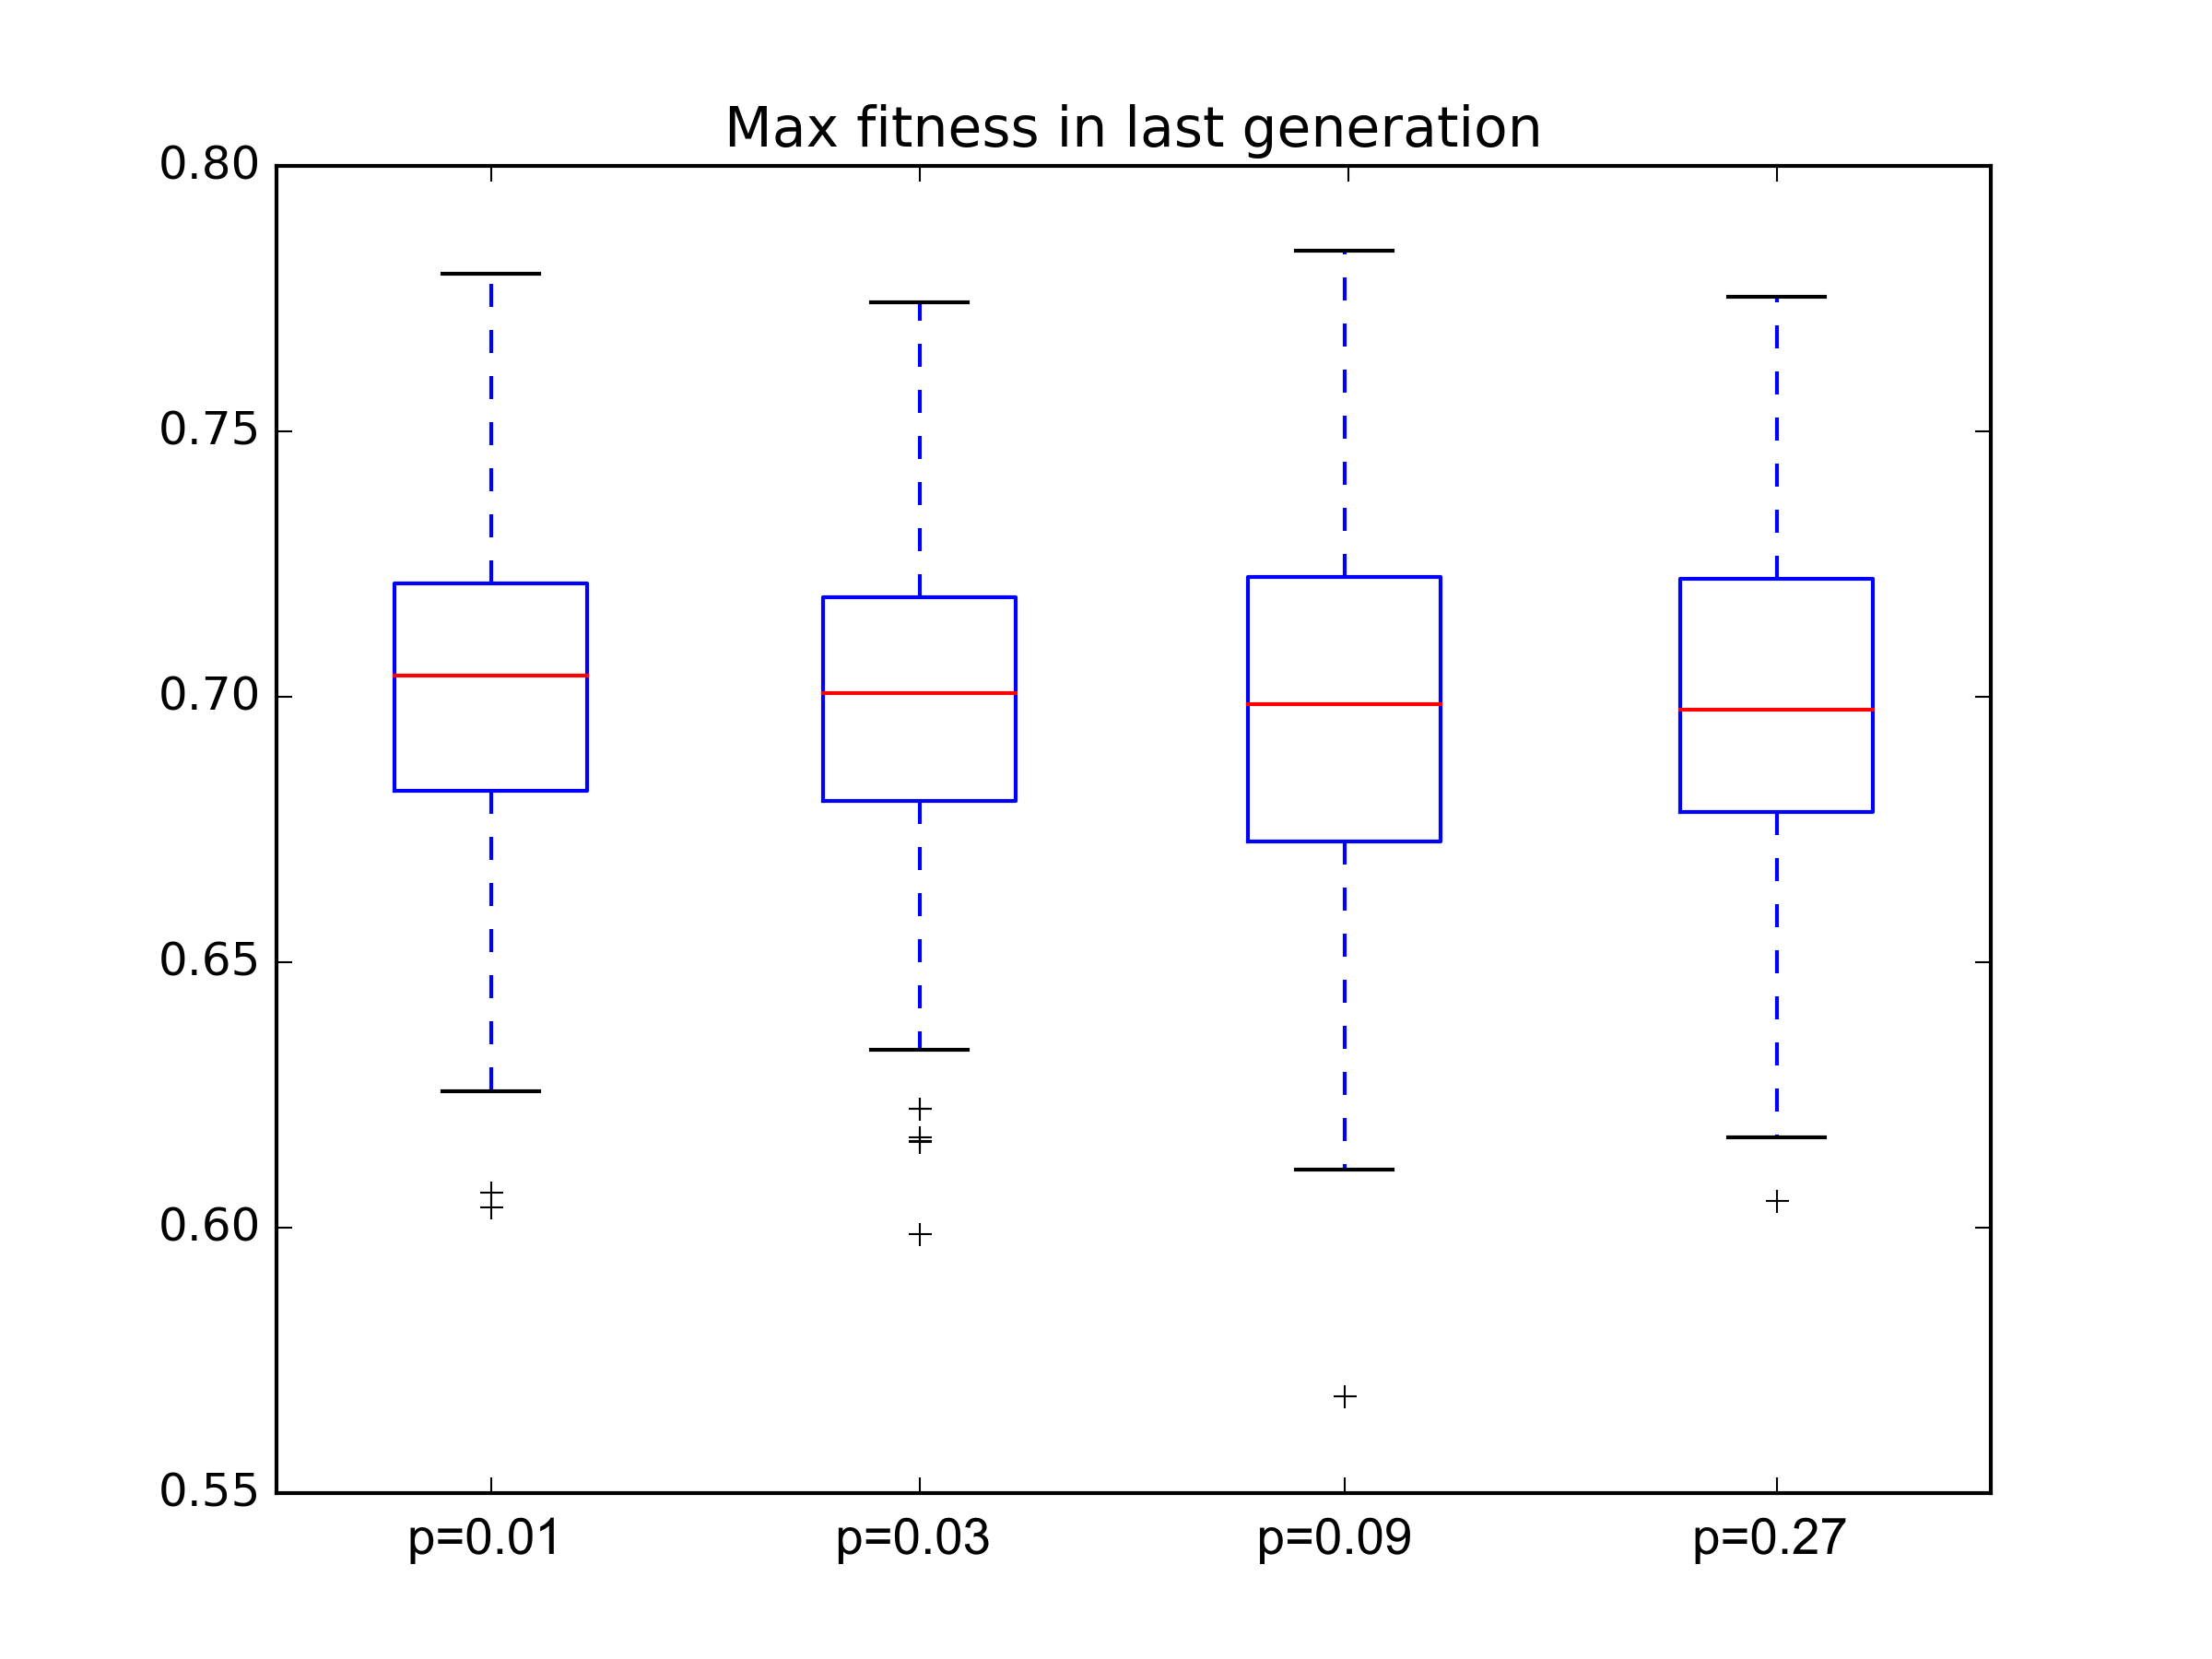
\includegraphics[width=1.0\textwidth]{exp2_box}
    \caption{Box plot of fitness values in the 50th generation for each configuration}
    \label{fig:exp2_box}
\end{figure}

The median values in figure \ref{fig:exp2_box} are not solid evidence that one configuration is better than another. However, figure \ref{fig:exp2_add_remove_link_rates} shows that while all series converge to roughly the same average fitness value, $p=0.01$ yields the highest rate of convergence. In fact, as $p$ becomes larger, the rate of convergence declines. This might mean that the problem at hand is best solved with few or no hidden nodes. An alternative interpretation is that hidden nodes are useful, but that they slow down the search for the ultimate individual, due to increased complexity. In accordance with Occam's razor, the preferred choice is $p=0.01$, as it produces the neural networks with the simplest structures \citep{mitchell1997}.

\begin{figure}[H]
    \centering
    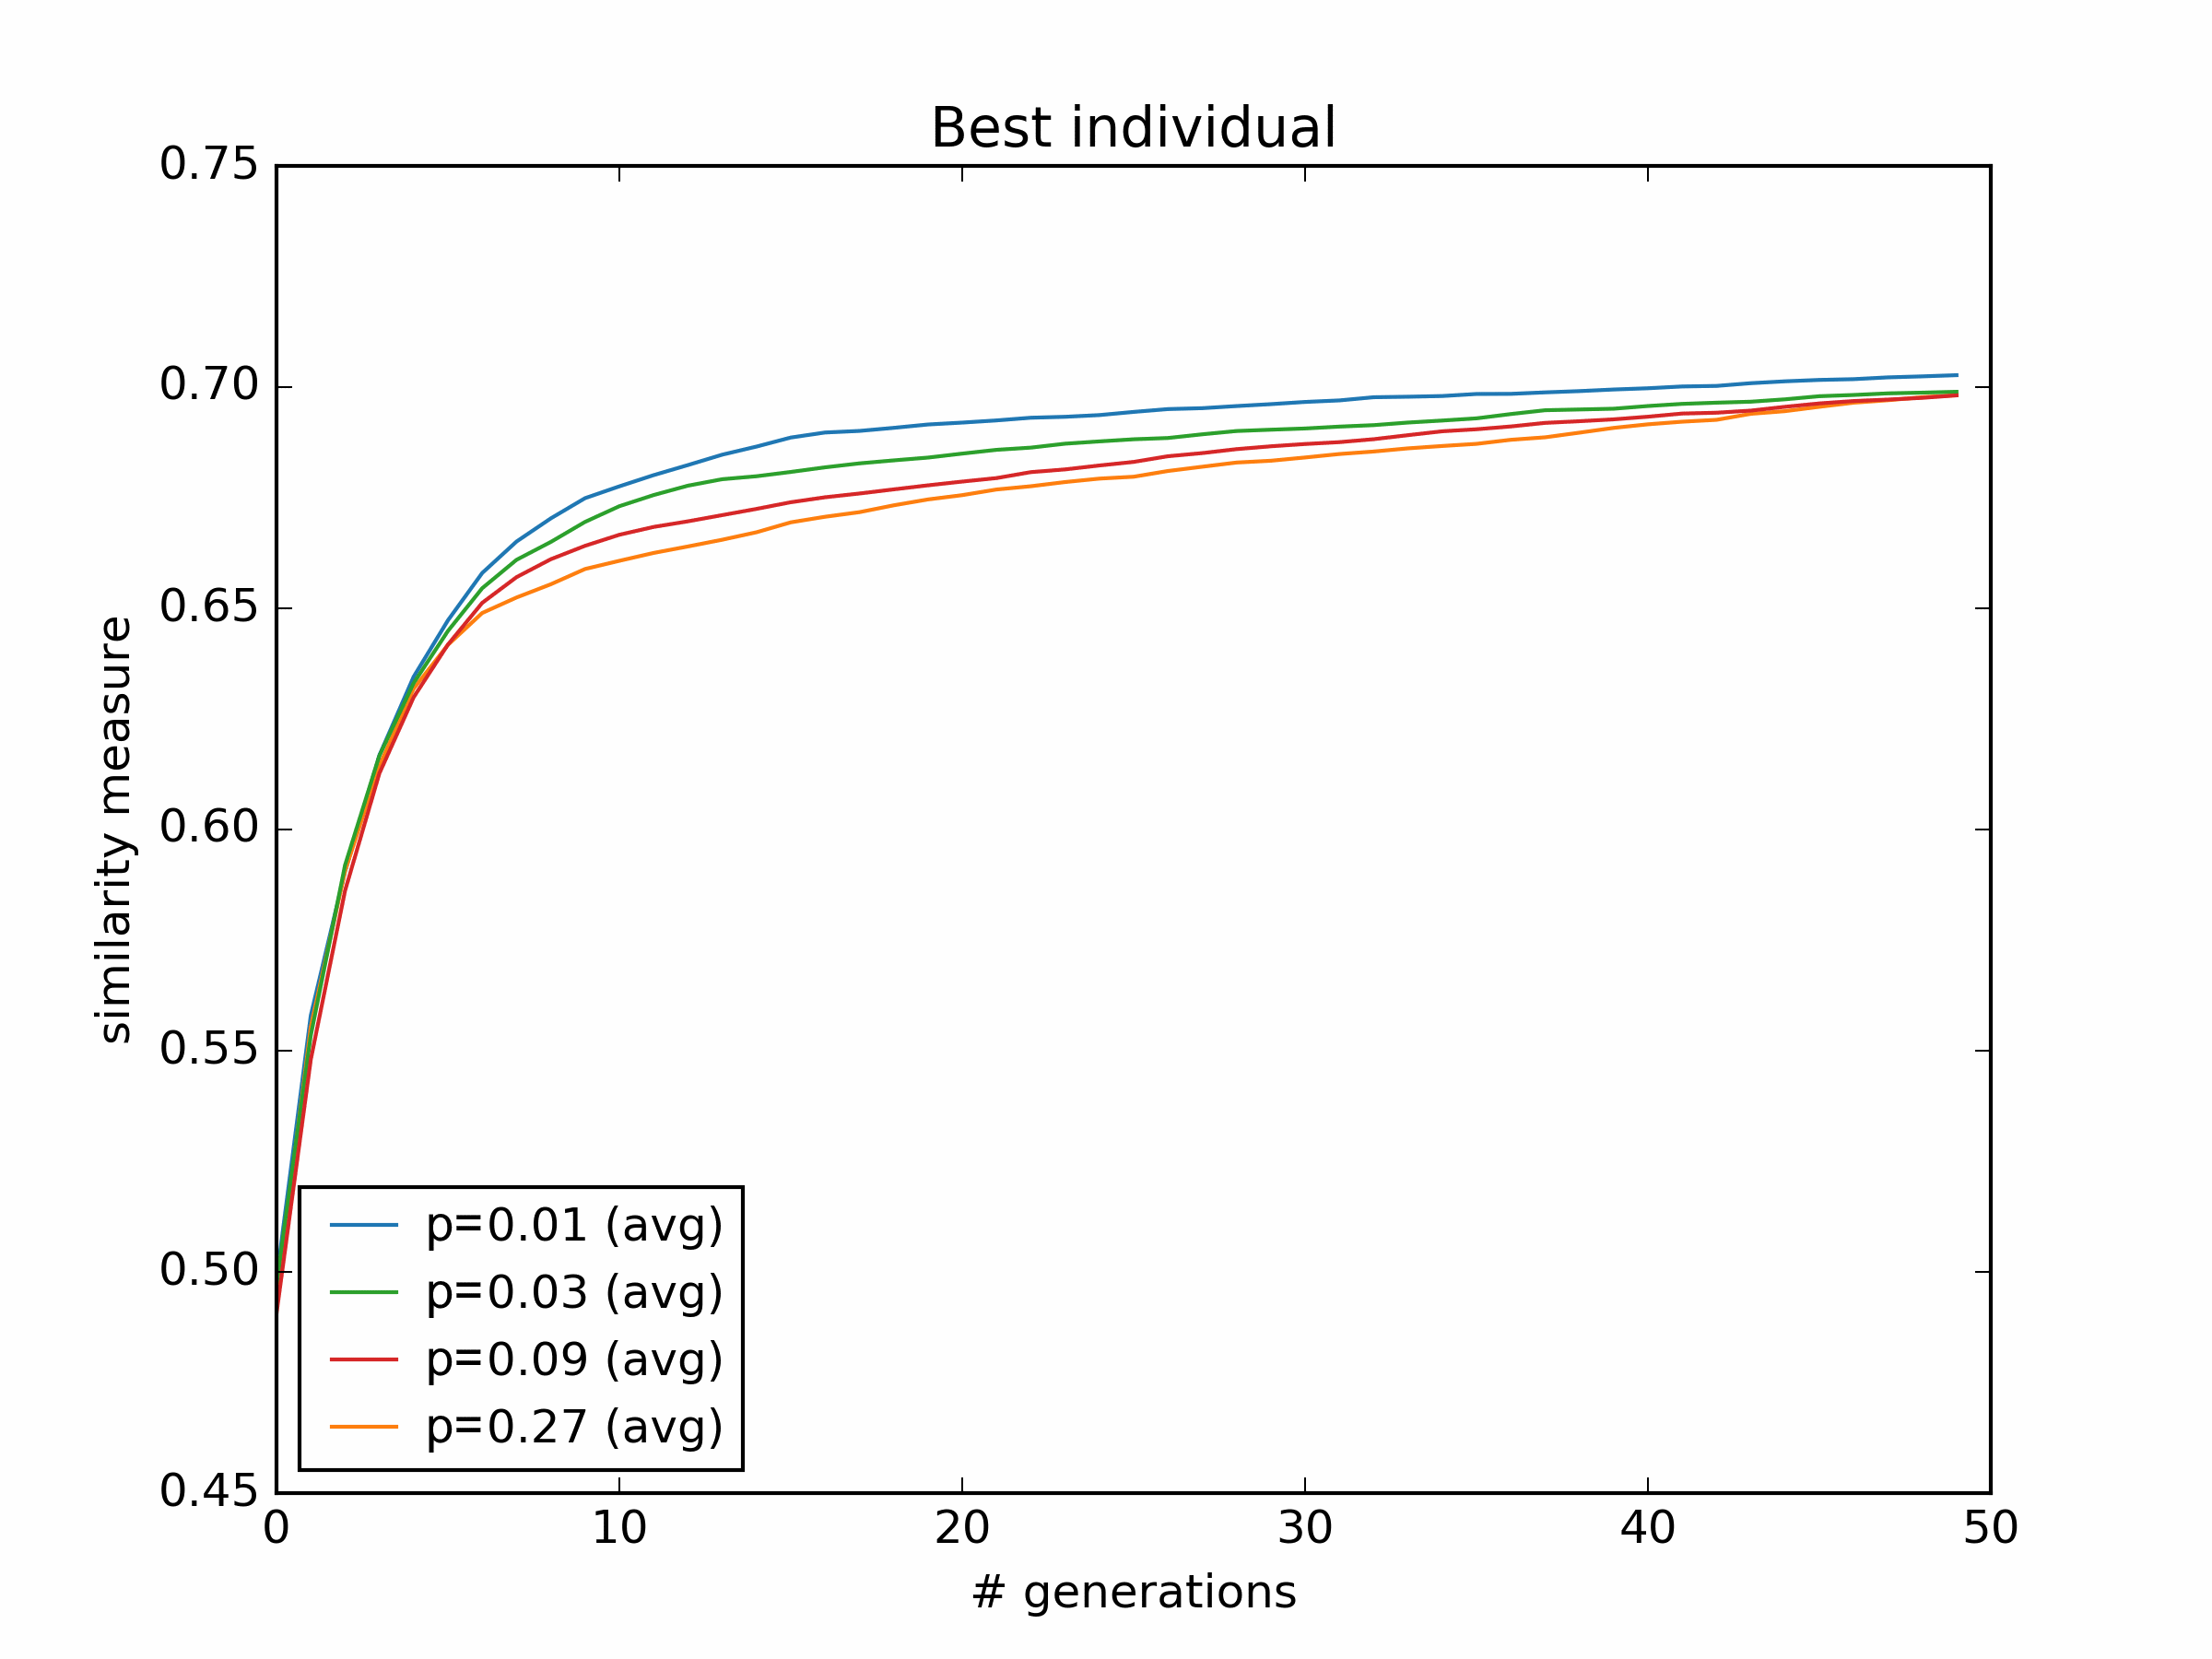
\includegraphics[width=1.0\textwidth]{exp2_add_remove_link_rates}
    \caption{Line chart showing the average fitness values in each generation}
    \label{fig:exp2_add_remove_link_rates}
\end{figure}

% TODO: Show typical end-result neural networks from all the configurations, to highlight that higher probability builds a larger, more complex network
